%
% File    : sample_4yp_report.tex
% Author  : Mauricio Villarroel
% Created : Apr 10, 2019
% ____________________________________________________________________________
%
% This program is free software; you can redistribute it and/or modify it
% under the terms of the GNU General Public License as published by the
% Free Software Foundation; either version 2 of the License.
%
% This program is distributed in the hope that it will be useful, but
% WITHOUT ANY WARRANTY; without even the implied warranty of
% MERCHANTABILITY or FITNESS FOR A PARTICULAR PURPOSE. See the GNU General
% Public License for more details.
% ____________________________________________________________________________
%
% DESCRIPTION :
%
% Sample 4YP Report of the Engineering department of 
% the University of Oxford
% ____________________________________________________________________________


\documentclass{4ypdocument}

\makeglossaries
\include{glossary}

%
% Project author and metadata
%

\title     {Your title}
\author    {Author's name}
\college   {Your college name}
\university{University of Oxford}
\universitylogo{oxford-logo}       % File name of the logo
\supervisor{Supervisor's name}
\degreedate{Hilary Term, 2048}

%
% Document contents
%

\begin{document}

\frontmatter

\maketitle

% Comment the following lines if writing a small progress report
\include{declaration}
\include{dedication}
\include{acknowledgements}
\include{abstract}

\tableofcontents
\listoffigures
\listoftables
\listofabbreviations

\mainmatter

%\layout  %Used temporarly for checking layout

\include{chap_introduction}
\include{chap_literature_review}
\chapter{Dataset}
\label{chapter:dataset} 


\section{Introduction}

\lipsum[2-4]

\section{Clinical study design}

\lipsum[2-4]

\section{Instrumentation}


\begin{figure}[tbh]
  \centering
  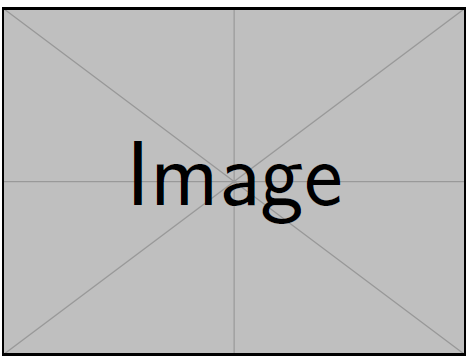
\includegraphics[width=0.9\linewidth,keepaspectratio=true]{dummy_image}
  \caption[Sample image]
  {
  Sample image.
  }
  \label{fig:sample_image}
\end{figure}

\Cref{fig:sample_image} shows the a dummy image ...


\lipsum[2-4]

\begin{figure}[tbh]
  \centering
  \subbottom[]{
    \label{fig:grasshopper:lens}
    \includegraphics[width=0.2\linewidth,keepaspectratio=true]{fujinon-hf125sa_lens}
  } 
  \subbottom[]{
    \label{fig:grasshopper:camera}
    \includegraphics[width=0.22\linewidth,keepaspectratio=true]{grasshopper2}
  }
  \subbottom[]{
    \label{fig:grasshopper:sensor}
    \includegraphics[width=0.45\linewidth,keepaspectratio=true]{grasshopper2_sensor}
  }
  \caption[The PointGrey Grasshopper2 video camera]
  {
  The video camera used in the study:
  \subcaptionref{fig:grasshopper:lens}   Fujinon HF12.5SA-1 lens,
  \subcaptionref{fig:grasshopper:camera} PointGrey Grasshopper2 camera module.
  \subcaptionref{fig:grasshopper:sensor} Response curve for the red, green and blue wavelengths from the image sensor inside the Grasshopper2 camera: Sony ICX625 2/3" progressive scan CCD (Source: PointGrey).
  }
  \label{fig:grasshopper}
\end{figure}

\Cref{fig:grasshopper} shows the video camera used in the study ...

\lipsum[2-4]

\Cref{table:grasshopper2_specs} describes the ...

\begin{table}[bth]
  \centering
  \caption[General features and specification for the PointGrey Grasshopper2 camera]
  {
  General features and specification for the PointGrey Grasshopper2 camera. (Source: PointGrey)}
  {\small
   \singleTableRowHeight
   \begin{tabular}{ll}
     \tableHeaderStart
        \tableHCell{Item} & \tableHCell{Description} \\
     \tableHeaderEnd
     Imaging Sensor        & Sony ICX625 2/3" progressive scan CCD \\
     Image size (pixels)   & 2448 (H) x 2048 (V)                   \\
     Pixel Size            & 3.45 \si{\micro\metre} x 3.45 \si{\micro\metre} \\
     A/D Converter         & AD9977 14-bit, dual-channel           \\
     Max frame rate        & 15 FPS                                \\
     Video Data Output     & 8, 12, 16 and 24-bit digital data     \\
     Gain \& Exposure                  & Automatic/Manual/One-Push              \\
     Lens Mount            & C-mount                                \\
     Interface             & Gigabit Ethernet                       \\
     Physical dimensions   & 44 (W) mm x 29 (H) mm x 58 (L) mm \\
     \hline 
   \end{tabular}
  }
  \label{table:grasshopper2_specs}
\end{table}

\lipsum[2-4]

\section{Patient population}

\lipsum[2-4]


\begin{table}[htb]
  \centering
  \caption{Summary of population demographics in the training and test sets}
  {
    \small
    \begin{tabular}{p{2cm} c c c c c c c c c c c}
      \toprule

      Set &
      \multirowcell{2}{Number of\\subjects} &
      \multirowcell{2}{Number of\\sessions} &
      \multirowcell{2}{Total time\\(hours)}$^1$ &
      \multicolumn{2}{c}{Gender} &      
      \multicolumn{6}{c}{Ethnicity$^2$}  \\

      \cmidrule{5-12}
        
      &   & &  & Male & Female & W & B & A & WB & WA & O  \\
      \midrule
      Training 	& 15 & 43 & 216.6 & 8  & 7  & 10 & 1   & 1 & 1 & 1 & 1 \\        
      Test 		& 15 & 47 & 210.0 & 10 & 5  & 10 & $-$ & 1 & 1 & 2 & 1 \\        
      \midrule        
      Total		& 30 & 90 & 426.6 & 18 & 12 & 20 & 1   & 2 & 2 & 3 & 2 \\
        
      \bottomrule
        
      \multicolumn{12}{l}
      {
        \footnotesize $^1$ Period during which both reference and estimated data were being recorded simultaneously.        
      } \\        
      \multicolumn{12}{l}
      {        
        \footnotesize $^2$ W = White, B = Black, A = Asian, WB = Mixed White \& Black, WA = Mixed White \& Asian and O = Other.        
      } \\
        
      \end{tabular}      
  } 
  \label{table:patient_demographics}
\end{table}

\subsection{Demographics}

The summary of the demographics for the entire set is described in  \cref{table:patient_demographics}. ...

\lipsum[2-4]

\subsection{Vital signs}

\lipsum[2-4]

\section{Conclusion}

\lipsum[2-4]
\include{chap_method_1}
\include{chap_method_2}
\include{chap_conclusion}

\appendix

\include{appendix_1}
\include{appendix_2}

\backmatter 

\listofreferences{references}

\end{document}
